% Created 2021-09-28 Tue 12:45
% Intended LaTeX compiler: xelatex
\documentclass[bigger]{beamer}
\usepackage{graphicx}
\usepackage{grffile}
\usepackage{longtable}
\usepackage{wrapfig}
\usepackage{rotating}
\usepackage[normalem]{ulem}
\usepackage{amsmath}
\usepackage{textcomp}
\usepackage{amssymb}
\usepackage{capt-of}
\usepackage{hyperref}
\usepackage{pifont}
\usepackage{verbatim}
\makeatletter
\def\verbatim@font{\scriptsize\ttfamily}
\makeatother
\logo{\includegraphics[height=0.5cm]{./img/usp-logo-1}}
\AtBeginSubsection[]{\begin{frame}\frametitle{Table of Contents}\tableofcontents[currentsection,currentsubsection]\end{frame}}
\usepackage{tikz}
\usetikzlibrary{arrows.meta}
\usetikzlibrary{positioning}
\usepackage{tcolorbox}
\tcbuselibrary{skins}
\usepackage{minted}
\usemintedstyle{lovelace}
\newenvironment{modern-quote}{\begin{itemize}}{\end{itemize}}
\tcolorboxenvironment{modern-quote}{blanker,before skip=6pt,after skip=6pt, borderline west={3mm}{0pt}{black!40!white}}
{\usebackgroundtemplate{\includegraphics[height=\paperheight]{./img/TP-yellow-34.jpg}}
\usetheme{}
\usecolortheme{magpie}
\date{  Universidade de São Paulo - DEMAR}
\title{O \LaTeX{}, uma roupagem moderna}
\author[Branquinho]{\textbf{Pedro Gomes Branquinho \\ \text{\scriptsize{pedro.branquinho@usp.br}}}}
\date[EEL-USP]{\textbf{\scriptsize{Mini-curso de \LaTeX} \\ Universidade de São Paulo - DEMAR}}
\useoutertheme[height=30pt]{sidebar}
\setbeamertemplate{frametitle}[sidebar theme]
\setbeamertemplate{itemize item}{\ding{166}}
\setbeamercolor{item projected}{bg=magenta!90!black,fg=white}
\setbeamertemplate{enumerate item}[circle]
\setbeamerfont{block title}{size={\centering}}
\setbeamercolor{block title}{bg=black!30!white,fg=white}
\hypersetup{
 pdfauthor={},
 pdftitle={O \LaTeX{}, uma roupagem moderna},
 pdfkeywords={},
 pdfsubject={},
 pdfcreator={Emacs 27.2 (Org mode 9.4.4)}, 
 pdflang={Portuguese}}
\begin{document}

\maketitle
\begin{frame}{Outline}
\tableofcontents
\end{frame}



\section{Setup do documento}
\label{sec:orge3e4a2a}
{\usebackgroundtemplate{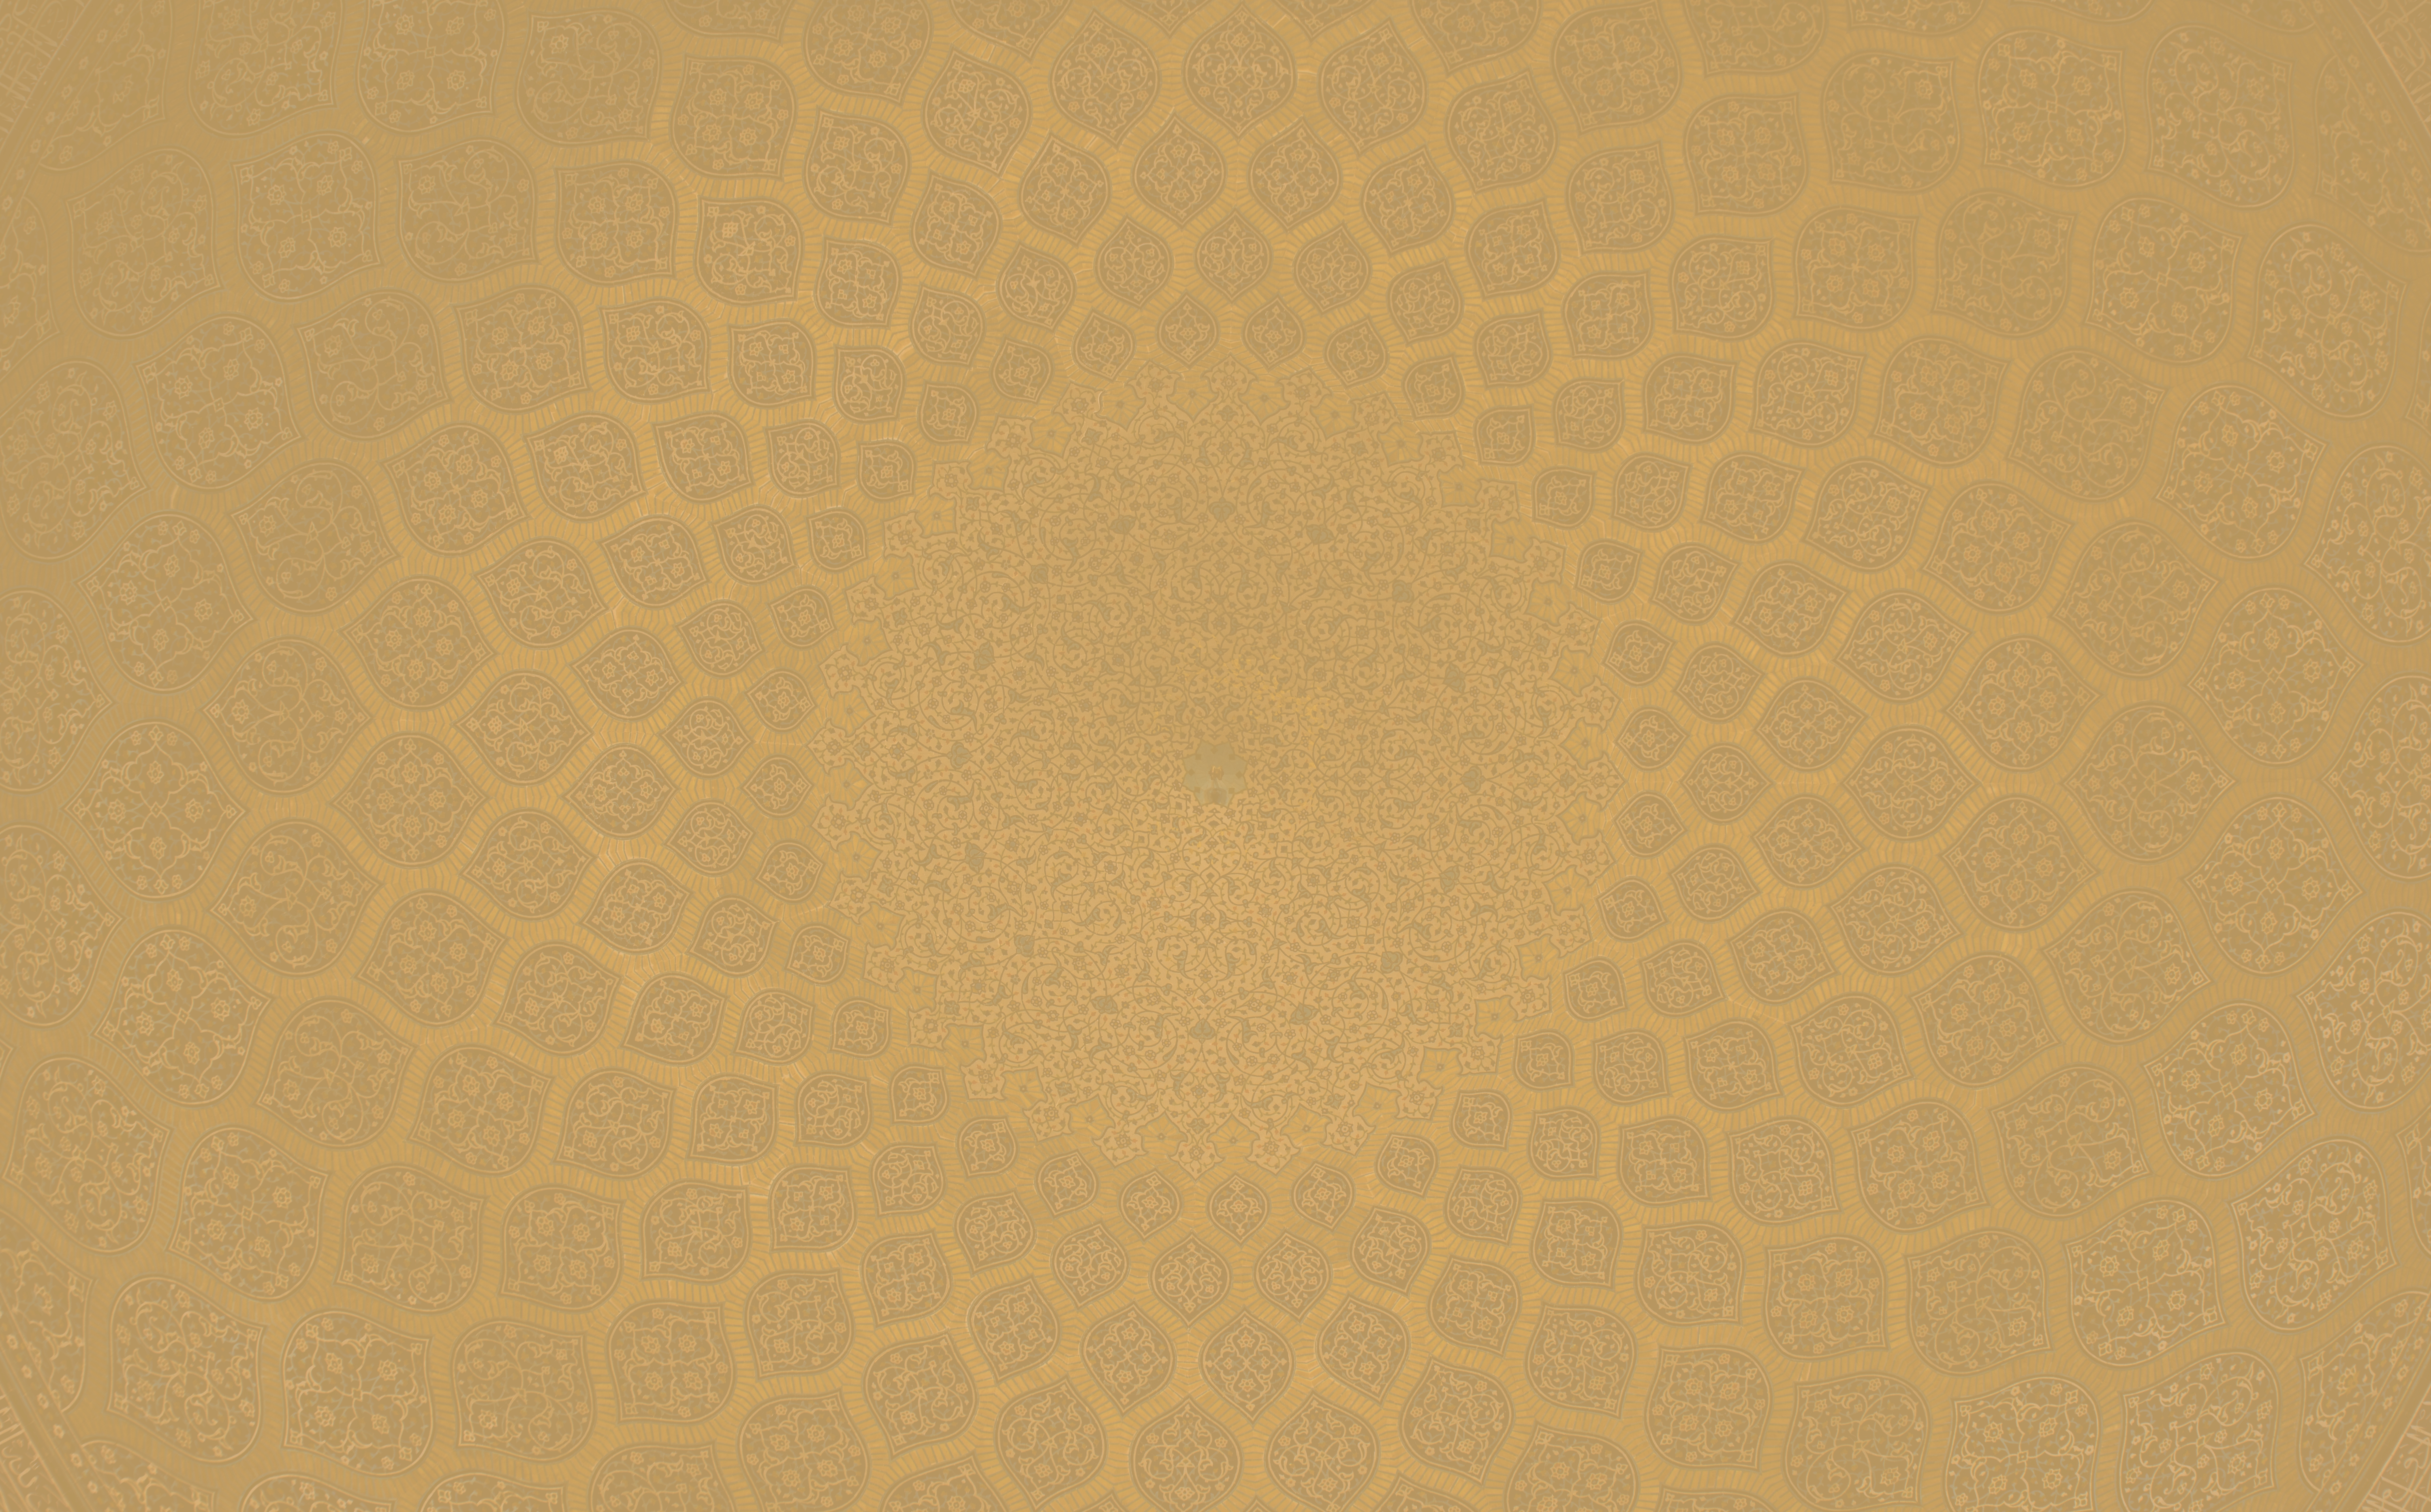
\includegraphics[height=\paperheight]{./img/yellow-30.jpg}}
\subsection{Estilização Beamer}
\label{sec:org9624a9b}
\begin{frame}[label={sec:org69aa734},fragile]{Preâmbulo org-mode}
 \begin{columns}
\begin{column}{0.92\columnwidth}
\begin{block}{Opções do Beamer}
\begin{minted}[fontsize=\scriptsize,autogobble=false,frame=lines,framesep=4pt,linenos=false]{latex}
\documentclass[bigger]{beamer} % espécide do documento
\useoutertheme[height=30pt]{sidebar} % disposição de itens
\setbeamertemplate{frametitle}[sidebar theme]
\usecolortheme{magpie} % Cor temática
\setbeamertemplate{itemize item}{\ding{166}} %Simb. item
\setbeamercolor{item projected}{bg=magenta!90!black,fg=white}
\setbeamertemplate{enumerate item}[circle] % Simb. enum.
\setbeamerfont{block title}{size={\centering}} % Tit. blocos
\setbeamercolor{block title}{bg=black!30!white,fg=white}
\end{minted}
\end{block}
\end{column}
\end{columns}
\end{frame}

\subsection{Minted (código)}
\label{sec:org4890997}
\begin{frame}[label={sec:org2357977},fragile]{Elisp}
 \begin{block}{Parâmetros \texttt{org-beamer-export}}
Dentro do Emacs, usando \texttt{emacs-lisp}
\begin{minted}[fontsize=\scriptsize,autogobble=false,frame=lines,framesep=4pt,linenos=false]{elisp}
(setq org-latex-listings 'minted)
(setq org-latex-minted-options
      '(("fontsize" "\\scriptsize")
	("autogobble" "false")
	("frame" "lines")
	("framesep" "4pt")
	("linenos" "false")))
\end{minted}
\end{block}
\end{frame}

\begin{frame}[label={sec:org8cae376},fragile]{\LaTeX{}}
 \begin{block}{Incluir \texttt{minted}}
Parte do preâmbulo,
\begin{minted}[fontsize=\scriptsize,autogobble=false,frame=lines,framesep=4pt,linenos=false]{latex}
\usepackage{minted}
\usemintedstyle{lovelace}
\end{minted}
\end{block}
\end{frame}
\section{Sumário de tópicos}
\label{sec:org0a68521}
\subsection{Pioneiros e Fundadores}
\label{sec:orgdff8101}
\begin{frame}[label={sec:org70f3669},fragile]{Origem de \TeX{} - Knuth (1978)}
 \begin{columns}
\begin{column}{0.48\columnwidth}
\begin{block}<1->{Imagem do Knuth}
\href{img/KnuthAtOpenContentAlliance.jpg}{\includegraphics[width=1.02\textwidth]{./img/KnuthAtOpenContentAlliance.jpg}}
\end{block}
\end{column}
\begin{column}{0.48\columnwidth}
\begin{block}<2>{Código Imagem}
\begin{minted}[fontsize=\scriptsize,autogobble=false,frame=lines,framesep=4pt,linenos=false]{latex}
\begin{figure}[!ht]
  \centering
  \includegraphics[width=\linewidth]
  {./img/Knuth.png}
\end{figure}
\end{minted}
\end{block}
\end{column}
\end{columns}
\end{frame}

\begin{frame}[label={sec:org60a9212}]{Origem de \TeX{} - Knuth (1978)}
\begin{columns}
\begin{column}{0.48\columnwidth}
\begin{block}{\small{~Ille eruditus et sapiens~}}
\href{img/KnuthAtOpenContentAlliance.jpg}{\includegraphics[width=1.02\textwidth]{./img/KnuthAtOpenContentAlliance.jpg}}
\end{block}
\end{column}

\begin{column}{0.52\columnwidth}
\begin{structureenv} %% Citação:
\begin{block}{\alert{\sout{\#AGORAVAI}}}
\begin{quote}
\textbf{"Só sei que nada sei..."}
\end{quote}
\begin{raggedleft}
\textbf{--- Albert Einstein}
\par\end{raggedleft}

\pause
\vspace{3mm}
\hline
\vspace{3mm}
\pause
\transboxin

\begin{modern-quote}
 \textbf{"Don't give up on your dreams, keep on sleeping."}
\end{modern-quote}
\begin{center}
--- Arthur 
\par\end{center}
\begin{raggedright}
Schopenhauer \pause \tikz[remember picture] \node [] (a)
\par\end{raggedright}

\begin{tikzpicture}[remember picture, overlay,
  every edge/.append style = {
    ->,
    thick,
    >=stealth,DimGray,
    dashed,
    line width = 1pt},  
  every node/.append style = {
    align = center,
    minimum height = 10pt,
    font = \bfseries,
    fill= green!20!white}]
  \node [right = 0.50cm of a, text width = 2cm] %and -.75 cm 
  (A) {Stonks};
  \draw (A.west) edge (a.west);
\end{tikzpicture}
\end{block}
\end{structureenv}
\end{column}
\end{columns}
\end{frame}


\begin{frame}[label={sec:orgd4872d2},fragile]{Roupagem moderna, \LaTeX{} - Leslie Lamport (1985)}
 \begin{columns}
\begin{column}{0.48\columnwidth}
\begin{block}<1->{Imagem Lamport}
\href{img/Leslie\_Lamport.jpg}{\includegraphics[width=1.02\textwidth]{./img/Leslie_Lamport.jpg}}
\pause
\transblindshorizontal[duration=0.8]
\end{block}
\end{column}
\begin{column}{0.48\columnwidth}
\begin{block}<1->{Código da Imagem}
\begin{minted}[fontsize=\scriptsize,autogobble=false,frame=lines,framesep=4pt,linenos=false]{latex}
\begin{figure}[!ht]
  \centering
  \includegraphics[width=\linewidth]
  {./img/Lamport.png}
\end{figure}
\end{minted}
\end{block}
\end{column}
\end{columns}
\end{frame}

\subsection{Aplicações que utilizam de \LaTeX{}}
\label{sec:org2a6a943}
\begin{frame}[label={sec:org2abb943}]{MathJax - \LaTeX{} na Web}
\transdissolve
\href{img/mathjax.png}{\includegraphics[center,width=1.02\textwidth]{./img/mathjax.png}}
\end{frame}

\begin{frame}[label={sec:org6c6003a},fragile]{Org-mode e AUCTeX (O código que usamos)}
 \begin{block}<1->{Código da Equação de Navier-Stokes}
\begin{minted}[fontsize=\scriptsize,autogobble=false,frame=lines,framesep=4pt,linenos=false]{latex}
\begin{equation}
	  \begin{aligned}
	  \dfrac{\partial{\vec{V}}}{\partial{t}}
	  + \vec{V}.\nabla{\vec{V}}
	  = - \dfrac{\nabla{p}}{\rho}
	  + \nu{}\nabla^2{\vec{V}}
	  \end{aligned}
  \end{equation}
\end{minted}

\transdissolve
\pause
\end{block}

\begin{block}<1->{Renderização Equação de Navier-Stokes}
\begin{equation}
        \begin{aligned}
        \dfrac{\partial{\vec{V}}}{\partial{t}} + \vec{V}.\nabla{\vec{V}} = - \dfrac{\nabla{p}}{\rho} + \nu{}\nabla^2{\vec{V}}
        \end{aligned}
\end{equation}
\end{block}
\end{frame}

\begin{frame}[label={sec:org515ff6e}]{Dentro do Org-mode, no Emacs}
\begin{itemize}[<+->]
\item Preview em tempo real.
\item Aparência customizável.
\item Ecossistema para programação.
\end{itemize}

\href{img/orgmode-auctex.png}{\includegraphics[center,width=0.8\textwidth]{./img/orgmode-auctex2.png}}
\end{frame}

\subsection{Sintaxe básica de listagem e enumeração}
\label{sec:org4997c80}
\begin{frame}[label={sec:org6f972da},fragile]{Itemize}
 \begin{columns}
\begin{column}{0.48\columnwidth}
\begin{block}<1->{Como renderiza:}
\begin{itemize}
\item Primeiro item
\item Segundo item
\end{itemize}
\end{block}
\end{column}

\begin{column}{0.48\columnwidth}
\begin{block}<2->{O código:}
\begin{minted}[fontsize=\scriptsize,autogobble=false,frame=lines,framesep=4pt,linenos=false]{latex}
\begin{enumerate}
\item Primeiro item
\item Segundo item
\end{enumerate}
\end{minted}
\end{block}
\end{column}
\end{columns}
\end{frame}

\begin{frame}[label={sec:orgebb4326},fragile]{Enumerate}
 \begin{columns}
\begin{column}{0.48\columnwidth}
\begin{block}<1->{Como renderiza:}
\begin{enumerate}
\item Primeiro item
\item Segundo item
\end{enumerate}
\end{block}
\end{column}
\begin{column}{0.48\columnwidth}
\begin{block}<2->{O código:}
\begin{verbatim}
\begin{enumerate}
\item Primeiro item
\item Segundo item
\end{enumerate}
\end{verbatim}
\end{block}
\end{column}
\end{columns}
\end{frame}

\subsection{Tabelas}
\label{sec:orgd304c87}
\begin{frame}[label={sec:orgc40ced9},fragile]{Tabela Simples}
 \begin{block}<1->{\small{Exemplo}}
\begin{center}
\begin{tabular}{lll}
\hline
Coluna 1 & Coluna 2 & Coluna 3\\
\hline
\(a_{11}\) & \(a_{12}\) & \(a_{13}\)\\
\(a_{21}\) & \(a_{22}\) & \(a_{23}\)\\
Texto 1 & Texto 2 & Texto 3\\
\hline
\end{tabular}
\end{center}
\end{block}

\begin{block}<2->{\small{Código}}
\begin{minted}[fontsize=\scriptsize,autogobble=false,frame=lines,framesep=4pt,linenos=false]{latex}
\begin{tabular}{lll}
  \hline
  Coluna 1 & Coluna 2 & Coluna 3\\
  \hline
  \(a_{11}\) & \(a_{12}\) & \(a_{13}\)\\
  \(a_{21}\) & \(a_{22}\) & \(a_{23}\)\\
  Texto 1 & Texto 2 & Texto 3\\
  \hline
\end{tabular}
\end{minted}
\end{block}
\end{frame}
\subsection{Exemplo de um documento completo}
\label{sec:org9f18cec}
\begin{frame}[label={sec:org1e4cf20},fragile]{Preâmbulo}
 \begin{block}{Preâmbulo mínimo}
\begin{itemize}
\item Onde fica as especificações da tipografia do documentos.
\item Ambiente mais genérico.
\item Onde os comportamentos padrões são especificados.
\end{itemize}
\end{block}

\begin{block}<2->{Definindo a classe do documento}
\begin{minted}[fontsize=\scriptsize,autogobble=false,frame=lines,framesep=4pt,linenos=false]{latex}
%!Tex TS-program = xelatex
%!TEX encoding = UTF-8 Unicode

  \documentclass[
  12pt, a4paper,		% tamanho da fonte e papel.
  openright,			% capítulos começam em pág ímpar (insere página vazia caso preciso)
  oneside,			% para impressão em recto somente. Oposto a twoside.
  brazil, english		% o último idioma é o principal do documento, ademais são hifenizados corretamente.
  ]{abntex2}
  \RequireXeTeX %Force XeTeX check
\end{minted}
\end{block}
\end{frame}

\begin{frame}[label={sec:orge44a230},fragile]{Os pacotes pertinentes}
 \begin{block}<1->{Alguns que definem fonte, indentação, etc.}
\begin{minted}[fontsize=\scriptsize,autogobble=false,frame=lines,framesep=4pt,linenos=false]{latex}
% --- (tudo que vem depois de '%' é um comentário em latex)
% ---
% Pacotes fundamentais 
% ---
\usepackage{lmodern}	% Usa a fonte Latin Modern
\usepackage[T1]{fontenc}% Seleção de codigos de fonte.
\usepackage[utf8]{inputenc}% Codificacao do documento (acentos)
\usepackage{indentfirst}% Indenta o primeiro parágrafo da secção.
\usepackage{color}% Controle das cores
\usepackage{graphicx}	% Inclusão de gráficos
\usepackage{microtype}% para melhorias de
% justificação
\usepackage{xltxtra} %fontspec, metalogo e realscripts (XeLaTex)
\usepackage{fontspec}
\usepackage{lipsum} % Enche linguíça (preenche espaço)
\usepackage[alf]{abntex2cite}% Citações padrão ABNT
\usepackage{amsmath} % Diversas tipografias matemáticas
\end{minted}
\end{block}
\end{frame}
\begin{frame}[label={sec:org6c805d8},fragile]{Corpo do documento}
 \begin{block}<1->{Um texto dentro do ambiente \texttt{document}}
\begin{minted}[fontsize=\scriptsize,autogobble=false,frame=lines,framesep=4pt,linenos=false]{latex}
\begin{document} %% Iniciar o documento

\chapter{Capítulo 1}
\section{Secção número 1.1}

\textbf{De acordo com \cite{knuth1984literate}, Literate programming
  é o paradigma mais formal e divertido de todos.}

\begin{figure}[ht]
  \centering
  \caption{\label{fig:lt1} Exemplo de literate programming.}
  \includegraphics[width=\linewidth]{./img/literate-programming.jpeg}
  \legend{Reference: The internet}
\end{figure}

\lipsum[1-2] % Texto enche linguíça

\bibliography{arquivo-com-bibliografias} % Usar bibliografias

\end{document}
\end{minted}
\end{block}
\end{frame}

\subsection{Código Tipografado}
\label{sec:org203b8d3}
\begin{frame}[label={sec:org1898994},fragile]{Python com \texttt{pygments}, usando \texttt{minted}}
 \begin{block}{Como renderiza}
\begin{minted}[fontsize=\scriptsize,autogobble=false,frame=lines,framesep=4pt,linenos=false]{python}
import numpy as np
\end{minted}

\begin{minted}[fontsize=\scriptsize,autogobble=false,frame=lines,framesep=4pt,linenos=false]{python}
np.sin(43)
\end{minted}

\begin{verbatim}
-0.8317747426285983
\end{verbatim}
\end{block}

\begin{block}{Código em \LaTeX{} (Minted e Pygments)}
\href{img/minted.png}{\includegraphics[width=0.8\textwidth]{./img/minted.png}}

\begin{minted}[fontsize=\scriptsize,autogobble=false,frame=lines,framesep=4pt,linenos=false]{latex}
\begin{verbatim}
 -0.8317747426285983
\end{verbatim}
\end{minted}
\end{block}
\end{frame}

\subsection{Referências}
\label{sec:org3ac931e}
\begin{frame}[label={sec:orgfb719e5}]{Documentação e modelos}
\begin{itemize}
\item \alert{Gerais:}
\begin{itemize}
\item Tikz: \url{https://latexdraw.com/}
\item Overleaf:
\end{itemize}

\item \alert{Minicursos}
\end{itemize}
\end{frame}
\end{document}